% This LaTeX was auto-generated from MATLAB code.
% To make changes, update the MATLAB code and export to LaTeX again.

\documentclass{article}

\usepackage[utf8]{inputenc}
\usepackage[T1]{fontenc}
\usepackage{lmodern}
\usepackage{graphicx}
\usepackage{color}
\usepackage{hyperref}
\usepackage{amsmath}
\usepackage{amsfonts}
\usepackage{epstopdf}
\usepackage[table]{xcolor}
\usepackage{matlab}

\sloppy
\epstopdfsetup{outdir=./}
\graphicspath{ {./classification_trees_images/} }

\begin{document}

\matlabtitle{Classification Trees}

\begin{matlabcode}
load fisheriris
f = figure;
gscatter(meas(:,1), meas(:,2), species,'rgb','o',5);
xlabel('Sepal length');
ylabel('Sepal width');
\end{matlabcode}
\begin{center}
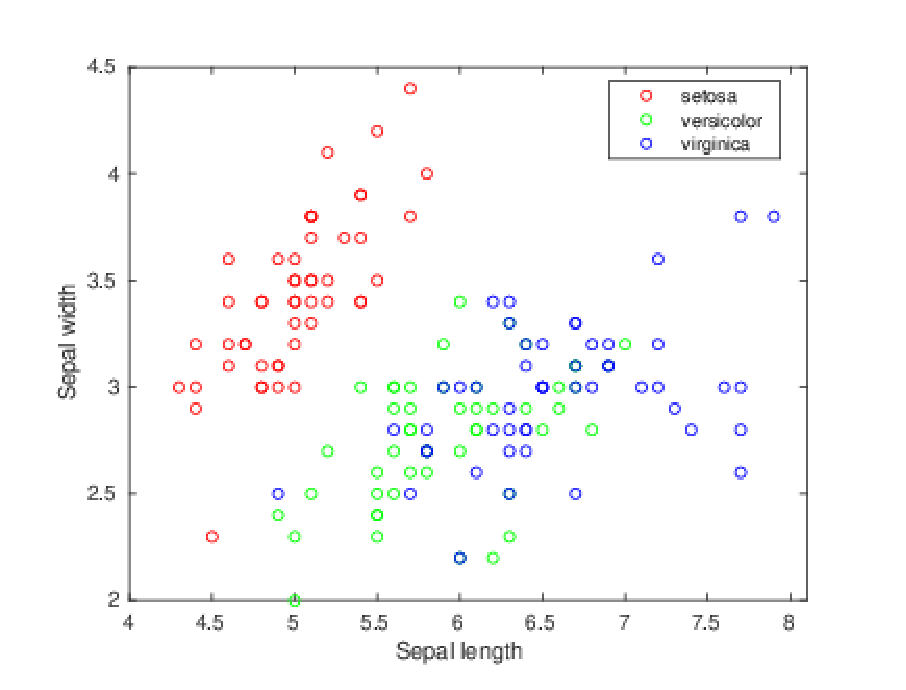
\includegraphics[width=\maxwidth{56.69844455594581em}]{figure_0.eps}
\end{center}

\begin{par}
\begin{flushleft}
Let's build a classification tree:
\end{flushleft}
\end{par}

\begin{matlabcode}
X = [ meas(:,1) meas(:,2)];
Y = species;

[bestFeature1, bestThreshold1, minGini1] = FindBestSplit(X,Y)
\end{matlabcode}
\begin{matlaboutput}
bestFeature1 = 1
bestThreshold1 = 5.4000
minGini1 = 0.4389
\end{matlaboutput}


\begin{matlabcode}
idx1 = X(:,bestFeature1)<=bestThreshold1;
idx2 = X(:,bestFeature1)>bestThreshold1;

X1 = X(idx1);
y1 = Y(idx1);
X2 = X(idx2);
y2 = Y(idx2);

[bestFeature11, bestThreshold11, minGini11] = FindBestSplit(X1,y1)
\end{matlabcode}
\begin{matlaboutput}
bestFeature11 = 1
bestThreshold11 = 4.8000
minGini11 = 0.2233
\end{matlaboutput}
\begin{matlabcode}
[bestFeature12, bestThreshold12, minGini12] = FindBestSplit(X2,y2)
\end{matlabcode}
\begin{matlaboutput}
bestFeature12 = 1
bestThreshold12 = 6.1000
minGini12 = 0.4546
\end{matlaboutput}


\begin{par}
\begin{flushleft}
We can draw the decision regions:
\end{flushleft}
\end{par}

\begin{matlabcode}
pred = Predict([0.1,0.5], bestFeature1, bestThreshold1, bestFeature11, bestThreshold11, bestFeature12, bestThreshold12, X1, y1, X2, y2)
\end{matlabcode}
\begin{matlaboutput}
pred = 
    {'setosa'}

\end{matlaboutput}
\begin{matlabcode}

figure;
[x,y] = meshgrid(4:.01:8,2:.01:4.5);
x = x(:);
y = y(:);
% Predict species for each point in the grid
j = arrayfun(@(idx) Predict([x(idx), y(idx)], bestFeature1, bestThreshold1, bestFeature11, bestThreshold11, bestFeature12, bestThreshold12, X1, y1, X2, y2), 1:length(x), 'UniformOutput', false);
j = [j{:}];

colors = [0 1 0; 1 0 0; 0 0 1];
face_alpha = 0.5;
\end{matlabcode}


\begin{matlabcode}
% Loop through unique species and plot points with custom colors and transparency
unique_species = {'versicolor','setosa','virginica'};
for i = 1:length(unique_species)
    scatter(x(strcmp(j, unique_species{i})), y(strcmp(j, unique_species{i})), [], colors(i,:), 'o', 'filled', 'MarkerFaceAlpha', face_alpha);
    hold on;
end
legend('versicolor','setosa','virginica')
\end{matlabcode}
\begin{center}
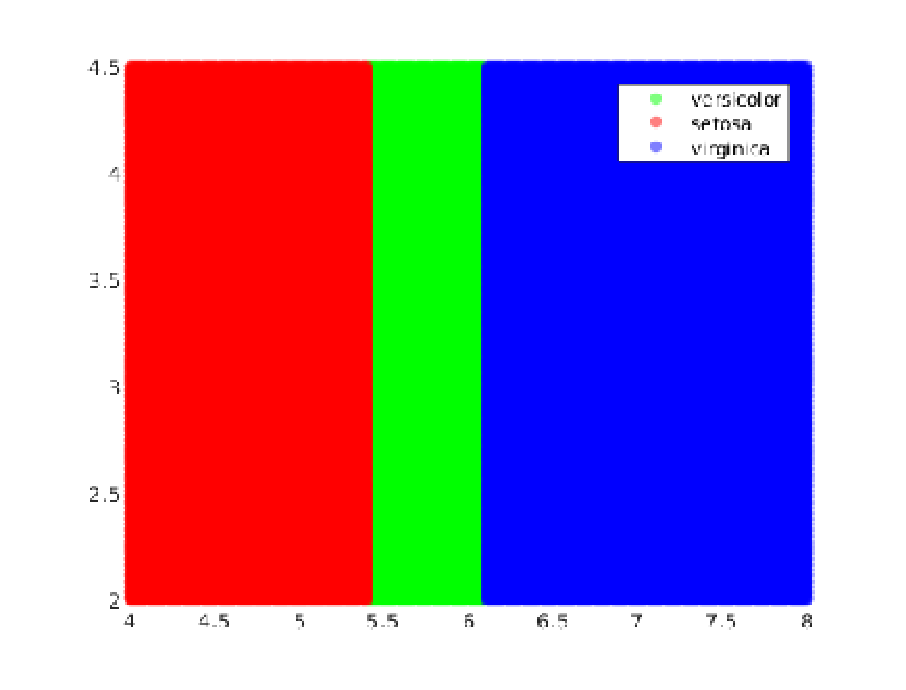
\includegraphics[width=\maxwidth{56.69844455594581em}]{figure_1.eps}
\end{center}

\begin{par}
\begin{flushleft}
As we can see, the result is not great, but this method can only divide the space in parallel hyperplanes to the axis. If we continued dividing the tree, we could improve the results. We can use the built-in trees to see what we can achieve:
\end{flushleft}
\end{par}


\begin{matlabcode}
Mdl = fitctree(X, Y, 'SplitCriterion', 'gdi'); % 'gdi' stands for Gini's diversity index
j = predict(Mdl, [x y]);

unique_species = {'versicolor','setosa','virginica'};
for i = 1:length(unique_species)
    scatter(x(strcmp(j, unique_species{i})), y(strcmp(j, unique_species{i})), [], colors(i,:), 'o', 'filled', 'MarkerFaceAlpha', face_alpha);
    hold on;
end
legend('versicolor','setosa','virginica')
\end{matlabcode}
\begin{center}
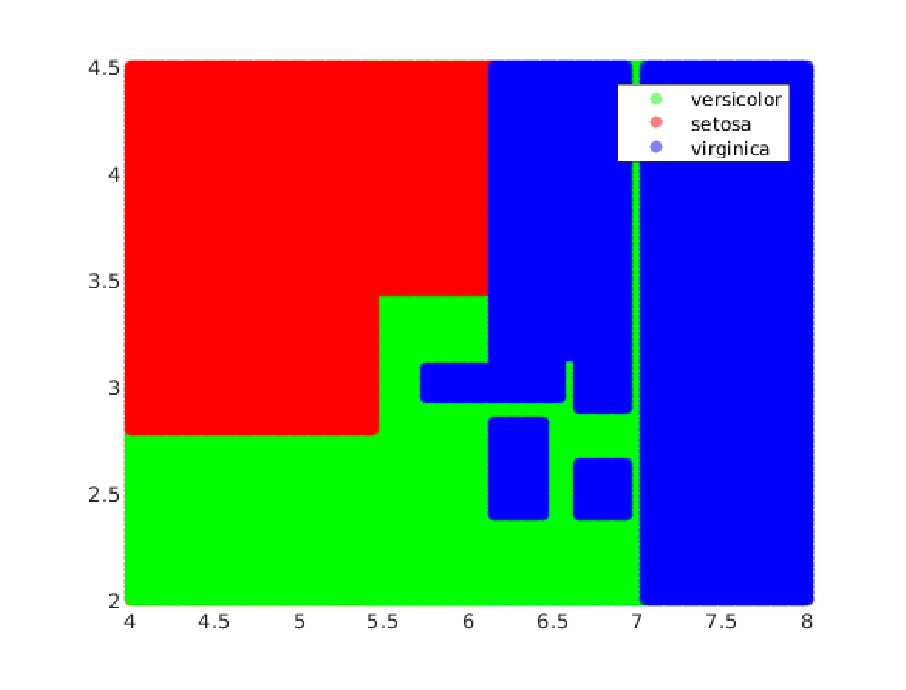
\includegraphics[width=\maxwidth{56.69844455594581em}]{figure_2.eps}
\end{center}

\begin{par}
\begin{flushleft}
This one seems to partition the space 'OK'.
\end{flushleft}
\end{par}


\begin{matlabcode}
function gini = GiniImpurity(y)
    K = unique(y);
    proportions = arrayfun(@(val) sum(strcmp(y,val))/numel(y), K);
    gini = 1 - sum(proportions.^2);
end

function [bestFeature, bestThreshold, minGini] = FindBestSplit(X, y)
    % Get number of instances and number of features
    [numInstances, numFeatures] = size(X);

    % Initialize bestFeature, bestThreshold, and minimum Gini impurity
    bestFeature = 0;
    bestThreshold = 0;
    minGini = Inf;

    % For each feature
    for feature = 1:numFeatures
        % For each possible threshold
        for threshold = 1:numInstances
            % Split data into two subsets
            subset1 = y(X(:, feature) <= X(threshold, feature));
            subset2 = y(X(:, feature) > X(threshold, feature));

            % Compute Gini impurities for the two subsets
            giniSubset1 = GiniImpurity(subset1);
            giniSubset2 = GiniImpurity(subset2);

            % Compute weighted Gini impurity
            gini = (numel(subset1) / numel(y)) * giniSubset1 + ...
                   (numel(subset2) / numel(y)) * giniSubset2;

            % If this split has a lower Gini impurity than the best one so far, update bestFeature, bestThreshold, and minGini
            if gini < minGini
                bestFeature = feature;
                bestThreshold = X(threshold, feature);
                minGini = gini;
            end
        end
    end
end

function prediction = Predict(x, bestFeature1, bestThreshold1, bestFeature11, bestThreshold11, bestFeature12, bestThreshold12, X1, y1, X2, y2)
    [y1_numeric, group_names1] = grp2idx(y1);
    [y2_numeric, group_names2] = grp2idx(y2);
    
    if x(bestFeature1) <= bestThreshold1
        if x(bestFeature11) <= bestThreshold11
            prediction_idx = mode(y1_numeric(X1(:,bestFeature11)<=bestThreshold11)); % Majority vote in leaf node
            prediction = group_names1(prediction_idx); % Convert back to label
        else
            prediction_idx = mode(y1_numeric(X1(:,bestFeature11)>bestThreshold11)); % Majority vote in leaf node
            prediction = group_names1(prediction_idx); % Convert back to label
        end
    else
        if x(bestFeature12) <= bestThreshold12
            prediction_idx = mode(y2_numeric(X2(:,bestFeature12)<=bestThreshold12)); % Majority vote in leaf node
            prediction = group_names2(prediction_idx); % Convert back to label
        else
            prediction_idx = mode(y2_numeric(X2(:,bestFeature12)>bestThreshold12)); % Majority vote in leaf node
            prediction = group_names2(prediction_idx); % Convert back to label
        end
    end
end

\end{matlabcode}

\end{document}
